\documentclass{article}

\usepackage{aligned-overset}
\usepackage{amsmath}
\usepackage{amssymb}
\usepackage{bbm}
\usepackage[shortlabels]{enumitem}
\usepackage{genealogytree}
\usepackage{hyperref}
\usepackage[utf8]{inputenc}
\usepackage{interval}
\intervalconfig{
  soft open fences
}

\usepackage{mathtools}
\usepackage{physics}
\usepackage{tikz}
\usetikzlibrary{patterns}
\usetikzlibrary{positioning}
\usetikzlibrary{shapes.geometric}
\usepackage{xcolor}
\definecolor{light-gray}{gray}{.9}

\author{Karsten Lehmann}
\date{03.11.2020}
\title{Übung Lineare Algebra - Grundlegende Konzepte}

\begin{document}


\maketitle
\newpage

\section*{Übung 1}
\begin{enumerate}
\item Für alle $a \in A \colon a \in B$ kann man auch schreiben als:
  \begin{enumerate}
  \item $A \cap B$
  \item $A = B$
  \item $A \subseteq B$
  \end{enumerate}
  \[
    \forall a \in A \colon a \in B \colon A \subseteq B
  \]
\item Welche der folgenden Terme ergibt eine leere Menge?
  \begin{enumerate}
  \item $A \cup B$
  \item $A \cap B$
  \item $A \setminus A$
  \end{enumerate}
\end{enumerate}

\section*{Übung 2}

Seien $A,B,C$ Mengen. Zeigen Sie

\begin{enumerate}
\item
  \[
    A \cap (B \cup C) = \color{blue} (A \cap B) \color{black} \cup \color{red} (A \cap C) 
  \]
  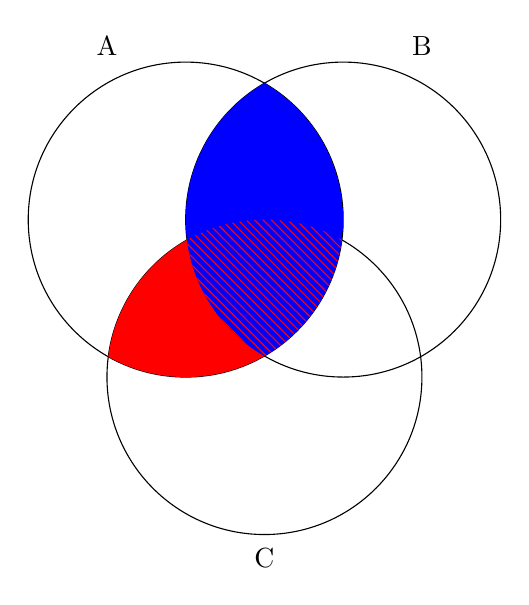
\begin{tikzpicture}    
    \def\circleA{(0,0) circle (2cm)}
    \def\circleB{(2,0) circle (2cm)}
    \def\circleC{(1,-2) circle (2cm)}

    \draw \circleA node[xshift=-1cm, yshift=2.2cm] {A};
    \draw \circleB node[xshift=1cm, yshift=2.2cm] {B};
    \draw \circleC node[yshift=-2.3cm] {C};

    %% Durchschnitt von A und C rot füllen
    \begin{scope}
      \clip \circleA;
      \clip \circleC;
      \fill[red] \circleA; 
    \end{scope}

    %% Durchschnitt von A und B blau füllen
    \begin{scope}
      \clip \circleA;
      \clip \circleB;
      \fill[blue] \circleA; 
    \end{scope}
    
    
    \begin{scope}
      \clip \circleB;
      \clip \circleC;
      \fill[preaction={fill=blue}, pattern color=red, pattern=north west lines] \circleA; 
    \end{scope}

  \end{tikzpicture}
\item
  \begin{align*}
    & A \cup (B \cap C) = (A \cup B) \cap (A \cup C)  \\
    x &\in (A  \cup B) \cap (A \cup C) \\
    &\iff x \in (A \cup B) \text{ und } x \in (A  \cup C) \\
    &\iff x \in A \text{ oder } x \in B \text{ und } x \in A \text{ oder } x \in C \\
    &\iff x \in A \text{ oder } x \in B \text{ und } x \in C \\
    &\iff x \in A \cup (B \cap C) \\
  \end{align*}
\end{enumerate}

\section*{Übung 3}

Seien $A, B$ Teilmengen einer Menge $X$. Zeigen Sie die Äquivalenz folgender Aussagen:

\begin{enumerate}
\item $A \cap B = \emptyset$
\item $A \subseteq X \setminus B$
\item $B \subseteq X \setminus A$
\end{enumerate}

\[
  X \setminus B \coloneqq \{ x \in X | x \notin B\}
\]

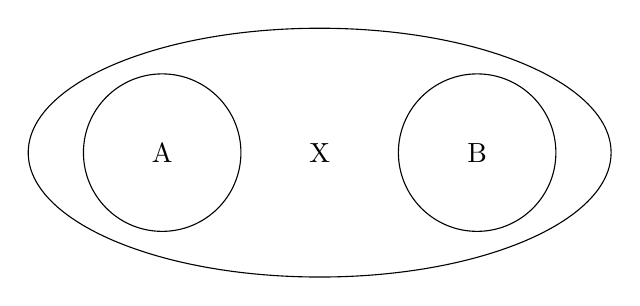
\begin{tikzpicture}
  \node[draw, ellipse, text height = 2cm, text width = 5cm] at (0,0) {};
  \node at (0,0) {X};
  \node[draw, circle, minimum size=2cm] at (-2,0) {A};
  \node[draw, circle, minimum size=2cm] at (2,0) {B};
\end{tikzpicture}

\section*{Übung 4}

Sei $M$ eine Menge und seien $A \subseteq M, B \subseteq M$. Wir bezeichnen mit $A^C$ das Komplement von $A$.
Finden Sie eine Menge $X \subseteq M$, die folgende Gleichung erfüllt:

\begin{align*}
  &(X \cup A)^C \cup (X \cup A^C)^C = B \\
  &m \in (X \cup A)^C \text{ oder } m \in (X \cup A^C)^C \\
  &\iff m \in M \setminus (X \cup A) \text{ oder } m \in M \setminus (X \cup A^C) \\
  &\iff m \in M \text{ und } m \notin (X \cup A) \text{ oder } m \in M \text{ und } m \notin (X \cup A^C) \\
  &\iff m \notin X \text{ oder } m \notin A \text{ oder } m \notin X \text{ oder } m \notin A^C \\
  &m \notin X \iff m \in B \\
  &\Rightarrow X = M \setminus B \\
\end{align*}

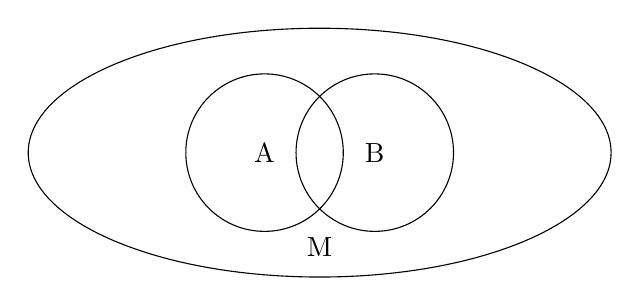
\begin{tikzpicture}
  \node[draw, ellipse, text height = 2cm, text width = 5cm] at (0,0) {};
  \node at (0,-1.2) {M};
  \node[draw, circle, minimum size=2cm] at (-.7,0) {A};
  \node[draw, circle, minimum size=2cm] at (.7,0) {B};
\end{tikzpicture}

\section*{Übung 6}

Sei $f \colon X \to Y$ eine Funktion und $A, B \subseteq X, C, D \subseteq Y$. Zeigen Sie die folgenden Aussagen

\begin{enumerate}
\item $f(A \cap B) \subseteq f(A) \cap f(B)$
\item $f(A \cup B) = f(A) \cup f(B)$
\item $X \setminus A \supseteq f(X) \setminus f(A)$
\item $f^{-1}(f(A)) \supseteq A$
\item $f^{-1}(C \cap D) = f^{-1}(C) \cap f^{-1}(D)$
\item $f^{-1}(C \cup D) = f^{-1}(C) \cup f^{-1}(D)$
\item $f^{-1}(Y \setminus C) = X \setminus f^{-1}(C)$
\item $f(f^{-1}(C)) \subseteq $
\end{enumerate}
\end{document}